\documentclass{article}

\usepackage{graphicx}
\usepackage{tikz}
\usepackage{tikzsymbols}
\usetikzlibrary{calc,patterns,shapes.geometric}
\pagestyle{empty}
\usepackage[margin=0pt]{geometry}
\geometry{papersize={14in,12in}}

\def\centerarc[#1](#2)(#3:#4:#5){\draw[#1] ($(#2)+({#5*cos(#3)},{#5*sin(#3)})$) arc (#3:#4:#5);}

\begin{document}
	\begin{figure}
		\centering
		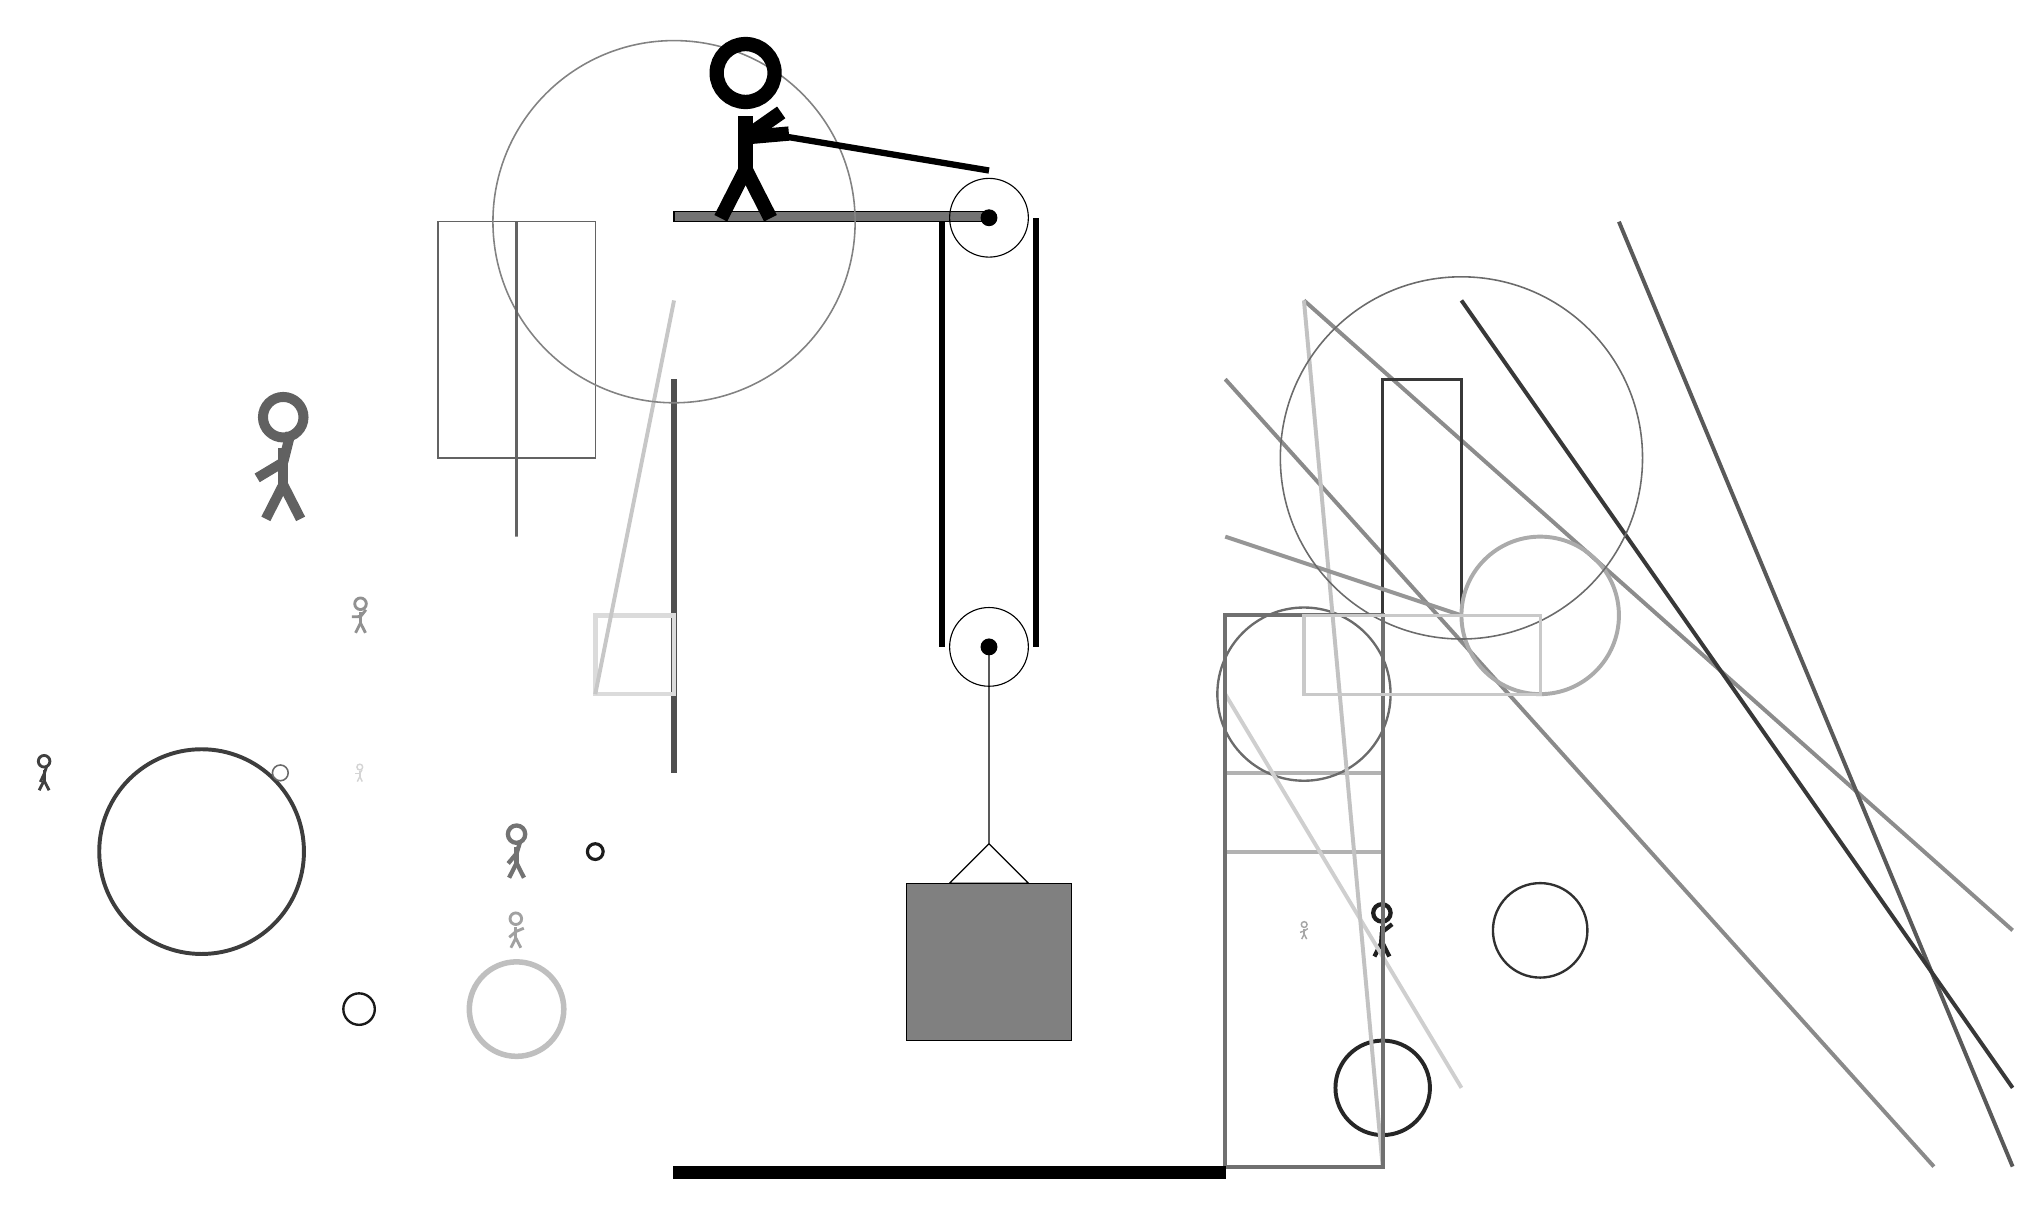
\begin{tikzpicture}
			%%%%% START %%%%%
			
			\draw[fill=black!55] (-2, 9) rectangle (2, 9.125);
			
			\draw (2, 3.6) circle (0.5);
			\draw[fill=black] (2, 3.6) circle (0.1);
			
			\draw (2, 9.05) circle (0.5);
			\draw[fill=black] (2, 9.05) circle (0.1);
			
			\node[line width=0.2mm, color=black!62] at (-7, 6) {\Strichmaxerl[7][31][76]};
			
			\draw [line width=0.3mm, color=black!90](-6, -1) circle (0.2);
			\draw[line width=0.5mm, color=black!46](5, 7) -- (14, -3);
			\draw[line width=0.7mm, color=black!69] (-2, 7) rectangle (-2, 2);
			\draw[line width=0.6mm, color=black!14] (-2, 4) rectangle (-3, 3);
			\draw[line width=0.5mm, color=black!45](6, 8) -- (15, 0);
			
			\draw[line width=0.5mm, color=black!30] (5, 2) rectangle (7, 1);
			
			\draw[line width=0.5mm, color=black!52] (-4, -1) rectangle (-4, -1);
			\draw [line width=0.5mm, color=black!85](7, -2) circle (0.6);
			
			\draw [line width=0.3mm, color=black!81](9, 0) circle (0.6);
			\node[line width=0.3mm, color=black!88] at (7, 0) {\Strichmaxerl[3][86][38]};
			\draw [line width=0.7mm, color=black!25](-4, -1) circle (0.6);
			\node[line width=0.2mm, color=black!35] at (6, 0) {\Strichmaxerl[1][19][33]};
			\node[line width=0.3mm, color=black!17] at (-6, 2) {\Strichmaxerl[1][0][60]};
			\draw[line width=0.5mm, color=black!22](-2, 8) -- (-3, 3);
			\draw [line width=0.4mm, color=black!89](-3, 1) circle (0.1);
			
			\draw [line width=0.3mm, color=black!58](6, 3) circle (1.1);
			
			\draw[line width=0.5mm, color=black!65](10, 9) -- (15, -3);
			\draw[line width=0.5mm, color=black!19](8, -2) -- (5, 3);
			\node[line width=0.5mm, color=black!75] at (-10, 2) {\Strichmaxerl[2][64][72]};
			\draw[line width=0.2mm, color=black!61] (-3, 6) rectangle (-5, 9);
			
			\node[line width=0.3mm, color=black!55] at (-4, 1) {\Strichmaxerl[3][50][73]};
			
			\draw[line width=0.5mm, color=black!24](7, -3) -- (6, 8);
			\node[line width=0.6mm, color=black!37] at (-4, 0) {\Strichmaxerl[2][41][23]};
			\draw [line width=0.2mm, color=black!49](-2, 9) circle (2.3);
			
			\draw[line width=0.4mm, color=black!78] (7, 7) rectangle (8, 4);
			\draw[line width=0.5mm, color=black!41](5, 5) -- (8, 4);
			\draw [line width=0.5mm, color=black!33](9, 4) circle (1.0);
			\node[line width=0.7mm, color=black!43] at (-6, 4) {\Strichmaxerl[2][1][52]};
			\draw[line width=0.5mm, color=black!78](8, 8) -- (15, -2);
			\draw[line width=0.3mm, color=black!61] (-4, 5) rectangle (-4, 9);
			
			\draw [line width=0.2mm, color=black!58](8, 6) circle (2.3);
			\draw [line width=0.5mm, color=black!76](-8, 1) circle (1.3);
			\draw [line width=0.2mm, color=black!59](-7, 2) circle (0.1);
			\draw[line width=0.5mm, color=black!56] (5, 4) rectangle (7, -3);
			\draw[line width=0.4mm, color=black!21] (6, 4) rectangle (9, 3);
			
			\draw (2, 3.6) -- (2, 1.1) -- (1.5, 0.6) -- (2.5, 0.6) -- (2, 1.1);
			\draw[fill=black!50] (0.95, 0.6) rectangle (3.05, -1.4);
			
			\draw[line width=0.8mm] (1.4, 9) -- (1.4, 3.6);
			\centerarc[line width=0.8mm](2, 3.6)(180:360:0.6);
			\draw[line width=0.8mm](2.6, 3.6) -- (2.6, 9.05);
			\centerarc[line width=0.8mm](2, 9.05)(0:90:0.6);
			\draw[line width=0.8mm](2, 9.65) -- (-1, 10.15);
			
			\node at (-1, 10.15) {\Strichmaxerl[10][-175][35]};
			
			\draw[fill=black] (-2, -3) rectangle (5, -3.15);
			
			%%%%% END %%%%%
		\end{tikzpicture}
	\end{figure}	
\end{document}